\textbf{ID:} UC12 (Delete Post) \\
\textbf{Scope:} CS Automated Information Timeline \\
\textbf{Level:} User goal \\
\textbf{Primary Actor:} Faculty or Admin/Reviewer \\
\textbf{Stakeholders and Interests: }
\begin{itemize}
    \item Audience: A person that is interested in viewing all approved content on the system using their mobile device.
    \item Faculty: A person that works for the university and is interested in gaining visibility of their post and/or event.
    \item Office Manager: A person that works for the university and is interested in prioritizing the order of posts and/or events.
    \item Admin/Reviewer: A person that works for the university and approves and/or removes posts and/or events from the system.
\end{itemize}
\textbf{Preconditions:}
\begin{itemize}
    \item Faculty has been identified and authenticated.
    \item A post to be deleted exists.
\end{itemize}
\textbf{Postconditions:}
\begin{itemize}
    \item The post has been deleted from the database.
    \item Media library has been updated.
    \item The display board no longer displays the deleted post.
\end{itemize}
\textbf{Main Success Scenario: }
\begin{enumerate}
    \item User navigates to the admin dashboard and accesses the manage post view.
    \item User selects the post to be managed and clicks the delete post button.
    \item System presents the confirmation window prompting the user if they are sure about deleting the post
    \item User confirms deletion.
    \item The system deletes the selected post from the database and updates the display board contents.
    \item System presents the confirmation that the post is deleted
\end{enumerate}
\textbf{Alternative Flows: } \\
a. At any time, system fails or becomes unresponsive and does not provide an error message
\begin{enumerate}
    \item User performs a hard refresh on the browser (ctrl + f5 or shift + reload)
    \item System reloads the editable view for the post
\end{enumerate}
b. (4.a) User does not confirm post deletion (clicks no)
\begin{enumerate}
    \item No action is taken, and the post is displayed in manage post view
\end{enumerate}

\begin{figure}[H]
    \centering
    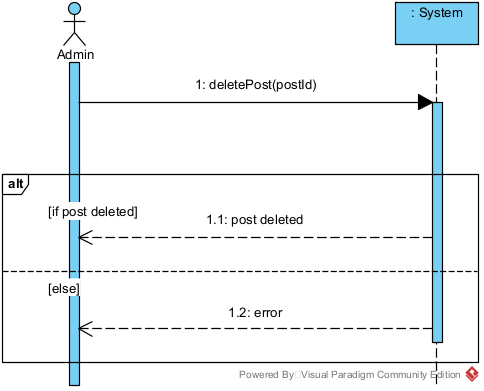
\includegraphics[width=0.8\textwidth]{images/SSD-UC12-DeletePost.png}
    \centering
    \caption{System Sequence Diagram: Delete Post}
\end{figure}

\textbf{Operation:} deletePost(postId) \\
\textbf{Cross Reference:} UC12  (Delete Post) \\
\textbf{Preconditions:}
\begin{itemize}
    \item Faculty has been identified and authenticated.
    \item A post has been created and persisted in the database.
    \item Delete operation is underway.
\end{itemize}
\textbf{Postconditions:}
\begin{itemize}
    \item A Post instance, post was created
    \item post was associated with the Delete operation.
    \item post was deleted
\end{itemize}